\clearpage

\def\chaptertitle{Background}

\lhead{\emph{\chaptertitle}}

\chapter{\chaptertitle}
\label{ch:background}

In this chapter, a brief introduction to Service Level Agreements is provided in section \ref{sec:sla}, followed by an overview of microservice architectures is provided in section \ref{sec:micro-svc-arc}. This includes a brief description of the architecture of Kubernetes, along with its scheduling and autoscaling algorithms. Finally, section \ref{sec:ch2-lit-review} comprises of a detailed literature review of the state-of-the-art autoscaling algorithms and a comparison of their performances and drawbacks.

\section{Service Level Agreements}
\label{sec:sla}

\begin{figure}[htb]
    \centering
    \caption{Types of service level agreements}
    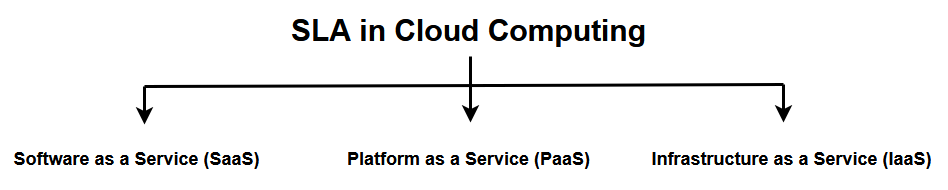
\includegraphics[width=0.9\linewidth]{Figures/SLA-Cloud-Computing.png}
    \label{fig:sla-types}
\end{figure}

Cloud computing generally exposes resource using a pay-as-you-go service. These lucrative plans have led to the implementation of applications and hardwares being delivered as Software as a Service (SaaS), Platform as a Service (PaaS), and Infrastructure as a Service (IaaS). However, consumers of such services have demands which may vary significantly, and it is impossible to fulfill all these expectations. Thus a balance needed to be struck in order to commit to an agreement \cite{patel2009service}. \par
This commitment is known as a Service Level Agreement (SLA). This SLA defines the expected services provided by the provider, and agreed to by the consumer. The most common metric by which SLAs are negotiated between providers and consumers is the availability of service.

\subsection{Availability of Services}
\label{subsec:svc-availability}
Availability is defined to ensure that the functional performance of the edge deployment is maintained for an agreed period. SLAs mostly define either monthly or yearly downtime in order to compute service credits for billing purposes \cite{mirobi2015service}. The downtime can be calculated using the formulae:
%TC:ignore
\[ downtime_{monthly} = \frac{100 - Availability\%}{100} * 30 * 24 \]
\[ downtime_{yearly} = \frac{100 - Availability\%}{100} * 365 \]
%TC:endignore
Table \ref{table:sla-availability} shows the expected down-times for several SLA availability percentages.

%TC:ignore
\begin{table}
    \caption{Summary of SLA availability}\label{table:sla-availability}
    \centering
    \begin{tabular}{|l|l|l|}
        \hline
        Availability \% & Monthly Downtime & Yearly Downtime\\
        \hline
        90\% & 72 hours & 36.5 days\\
        99\% & 7.2 hours & 3.65 days\\
        99.9\% & 43.8 minutes & 8.76 hours\\
        99.99\% & 4.38 minutes & 52.56 minutes\\
        99.999\% & 25.9 seconds & 5.26 minutes\\
        \hline
    \end{tabular}
\end{table}
%TC:endignore

\section{Microservice Architecture}
\label{sec:micro-svc-arc}

Microservice architectures involve decomposing an application into several loosely coupled services, and deploying them on separate servers known as ``nodes''. These services communicate with each other through a lightweight framework such as RESTful APIs \cite{li2021understanding}. Within these services, application data and commands are stored and executed within ``containers''. Typically, these architectures provide scalability, as well as ease of deployment and modification. Availability however, remains an important concern for such deployments. For a deployment to be classified as ``highly available'', it must be accessible at least 99.999\% of the time. For example, a highly available search engine would only face 5 minutes of down time per year \cite{nabi2016availability}. Therefore, an orchestration mechanism is required to manage the deployment and communication of these containers.\par

\begin{figure}[htb]
    \centering
    \caption{Features of container orchestration}
    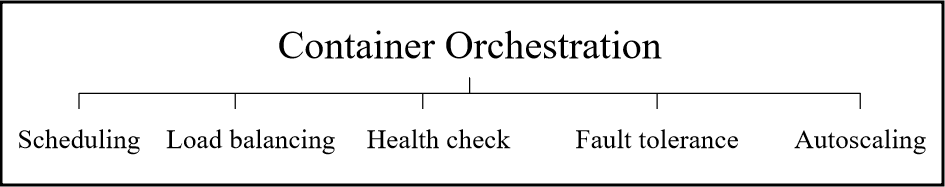
\includegraphics[width=0.9\linewidth]{Figures/Container-Orchestration.png}
    \label{fig:container-orchestration}
\end{figure}

Container orchestration allows the microservice application to customize how the deployment, monitoring, and controlling functions \cite{casalicchio2019container}. Figure \ref{fig:container-orchestration} depicts the typical features of container orchestration.\par
\textit{Scheduling} defines the rules on the number of containers to be executed at any given time. Scheduling also places containers on specific nodes based on availability and best performance.\par
\textit{Load balancing} distributes the resource usage among multiple microservice nodes. By default, a round-robin policy is implemented, although more complex policies may be implemented at the discretion of the developer.\par
\textit{Health checks} ensure that the container is still capable of responding to queries. Typically, these are done using a periodic light-weight HTTP request and verifying the response.\par
\textit{Fault tolerance} maintains several replicas of containers, a strategy commonly used to achieve the high availability mentioned above. Health checks are used to ensure the replicas are functioning, and they typically have strategies to ensure there is no mismatch in data between two fault tolerant containers.\par
\textit{Autoscaling} is the process of automatically adding or removing resources or containers. Internal metrics such as CPU usage are typically used, however custom policies can also be implemented at the discretion of the developer.\par

\subsection{Kubernetes Architecture}
\label{subsec:k8s-overview}

Kubernetes \footnote{\url{https://kubernetes.io/}} is one of the most popular open-source container orchestration platforms \cite{vayghan2019kubernetes}. Initially referred to as ``Borg'', the project was used internally at Google to deploy the majority of their cloud applications before becoming an open-source application \cite{burns2016borg}. Figure \ref{fig:k8s-arch} shows the high-level architecture. The Kubernetes deployment has a controller / worker architecture. The nodes in the Kubernetes cluster are split into either \textit{control plane nodes} and \textit{data plane nodes}. The \textit{control plane nodes} have a collection of processes which help monitor and maintain the desired state of the deployment. The \textit{data plane nodes} contain processes which run the containers doing the actual work, and are managed by the control plane.\par
The smallest unit of work in a Kubernetes deployment is known as a \textit{pod} \cite{baier2017getting}. This is a collection of containers sharing an IP address and port. In summary, microservice architectures are said to be containerized and deployed on Kubernetes in the form of pods \cite{vayghan2019kubernetes}.\par
\begin{figure}[htb]
    \centering
    \caption{Overview of Kubernetes architecture}
    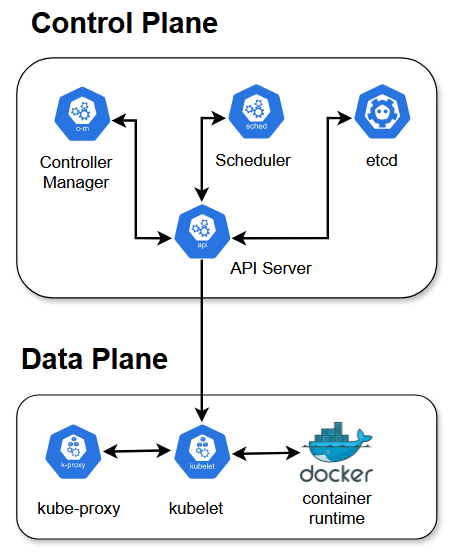
\includegraphics[width=0.5\linewidth]{Figures/K8s-Architecture.png}
    \label{fig:k8s-arch}
\end{figure}

\subsubsection{Data Plane}
\label{subsubsec:k8s-data-plane}

The \textit{container runtime} is a process which downloads or ``pulls'' the image for the required container onto the node. Kubernetes supports a wide range of runtimes, but some of the popular solutions are CRI-O \footnote{\url{https://cri-o.io/}}, containerd \footnote{\url{https://containerd.io/}}, and Docker \footnote{\url{https://www.docker.com/}}.\par

The most important process running on every data plane node is the \textit{kubelet}. This process executes the image assigned to the node via the container runtime, perform health checks, and reports the node status to the control plane.\par

Another data plane process is the \textit{kube-proxy}, which manages the rules for forwarding requests to services, as well as the IP tables of nodes. If a service is added or removed, kube-poxy updates the IP table accordingly.\par

\subsubsection{Control Plane}
\label{subsubsec:k8s-control-plane}
The \textit{API Server} is the primary communication endpoint for the entire deployment. Every component in the architecture communicates through it to exchange information. It is also used to update the current deployment state. The API Server is a simple RESTful API implementation, exposing well-documented APIs for access by other components as well as developers. Multiple replicas of this component are typically maintained to ensure high availability.\par

The \textit{etcd} is a data store which persists the deployment state in a key-value format. The data is serialized unlike in the stateless API server. This data adheres the properties of \textit{recovery} and \textit{availability}. \textit{Recovery} ensures that any corruption of data is reverted using a system of backups such as checkpoints. \textit{Availability} ensures that the deployment is reachable by the end-user regardless of the traffic being requested on the network.\par

\textit{Controller Manager} implements the desired deployment state. During initial deployment, the controller manager inputs the required workload as the desired state, after which it continually monitors the deployment state using a system of looping controls. If the deployment requires modifications, they are achieved using the API server, and the deployment is brought back into alignment with the desired state.\par

Finally, the \textit{scheduler} decides the location where the pod will be deployed. The scheduler runs a control loop which searches for uncheduled pods using the API server. It then assigns the pods to a dataplane node based on several predicates and priorities such as resource requirements and node affinity respectively.

\section{Autoscaling Overview}
\label{sec:autoscaling}

Apart from intelligently scheduling pods to data plane nodes \cite{kayal2020kubernetes}, Kubernetes has the provisions to dynamically respond to changes in resource requirements. This process of scaling nodes, pods, or other resources depending on requirements in an automated manner is known as \textit{autoscaling}. Kubernetes supports three variations of autoscaling.\par

\textit{Cluster autoscaling} modifies the number of nodes running in the entire deployment, or cluster. Dynamically allocating nodes based on resource requirements helps to manage the cost of running Kubernetes deployments on external platforms such as Amazon \footnote{\url{https://docs.aws.amazon.com/eks/}} or Google \footnote{\url{https://cloud.google.com/kubernetes-engine/}}. The autoscaler works by looping through two tasks. The first watches for unscheduled pods, the second checks if the current deployed pods (pods which are running on the data plane) can be merged on a smaller number of nodes.\par

\textit{Vertical pod autoscaling} modifies the CPU and memory resources assigned to pods. By default, the scheduler reserves a larger amount of these resources to pods than is usually required. By performing vertical pod autoscaling, the cluster can better manage its over-provisioned resources in real-time.\par

\textit{Horizontal pod autoscaling} is the most commonly used autoscaling strategy \cite{baresi2021kosmos}, it modifies the number of pods assigned to a task, based on the resources being requested. Kubernetes implements this using a periodic control loop which runs every 15 seconds by default. The control manager compares the actual resource utilization with the target utilization defined by the deployment script, and scales the number of pods accordingly.

\subsection{Custom Autoscaling}
\label{subsec:custom-autoscaling}

The default horizontal pod autoscaler uses pod CPU and memory utilization when making its scaling decisions. However, these metrics may be too rigid when it comes to edge architectures \cite{coulson2020adaptive}. The strict SLA constraints in place, along with the lower amount of resources present in the edge layer as compared to the cloud layer, make it imperative for custom metrics to be employed to autoscale resources as efficiently as possible.\par

Figure \ref{fig:custom-autoscale-overview} depicts the general architecture of the custom autoscaler. Typically, the autoscaler queries metrics from the default metrics registry, which acts as a central store for all metrics that are exposed to the developer. Three interfaces to this registry are exposed:
\begin{itemize}
    \item \textit{Resource metric API} is used to access predefined metrics such as CPU and memory resources of both pods as well as nodes.
    \item \textit{Custom metric API} contains user-defined custom metrics associated with all Kubernetes objects.
    \item \textit{External metrics API} contains metrics of objects which are not associated with Kubernetes.
\end{itemize}
For custom metric autoscaling, the autoscaler must be configured in a way where the metrics can be fetched from the custom metric API. This is done by configuring the custom metric server, several frameworks to simplify this process such as the Kubernetes Instrumentation SIG \footnote{\url{https://github.com/kubernetes/community/tree/master/sig-instrumentation}} exist which simplify the server building process.

\begin{figure}[htb]
    \centering
    \caption{Custom autoscaler architecture overview.}
    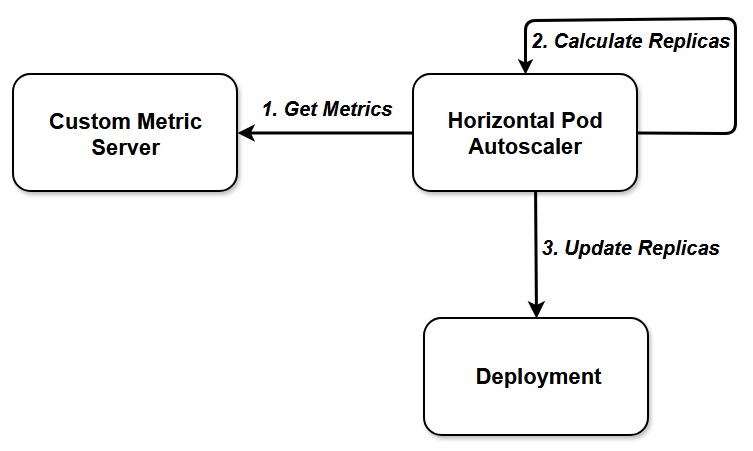
\includegraphics[width=.7\linewidth]{Figures/Custom-Metrics-Autoscaling.png}
    \label{fig:custom-autoscale-overview}
\end{figure}

\section{Time-Series Analysis}
\label{sec:ch2-time-series}

Several self-learning machine learning solutions exist. One of the most popular traditional models is the Convolutional Neural Network (CNN), which is a form of deep learning that attempts to learn data features through the process of filters optimization. However, while CNNs are excellent when working with 3-dimensional data such as images, it does not perform well when dealing with sequential inputs with interdependent data. Due to this, another machine learning subset known as Recurrent Neural Network (RNN) was conceptualized. \par

Recurrent Neural Networks store information about the past, and its future decisions are based on this information. Thus, while RNNs have a similar training process as CNNs, they remember features learned from prior inputs. RNNs are recurrent since they perform the same computation for each data element in the sequence, with each output being dependent on the previous computation. Figure \ref{fig:rnn-architecture} depicts this high-level architecture of the RNN.\par

\begin{figure}[htb]
    \centering
    \caption{Recurrent Neural Network Architecture}
    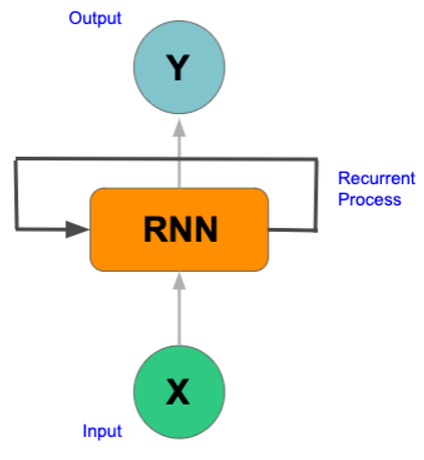
\includegraphics[width=.4\linewidth]{Figures/RNN-Overview.png}
    \label{fig:rnn-architecture}
\end{figure}

\suhrid{TODO: Unfold RNN image and show the image from intro to rnn page}

For the current RNN state, the formula can be written as follows:

\[ h_{t} = \mathcal{F}(h_{t-1}, x_{t})\]

Where $h_{t}$ is the current state, $h_{t-1}$ is the previous state, and $x_{t}$ is the current input value. In the simplest form, the function $\mathcal{F}$ is the activation function. Thus using the recurrent neuron weight $W_{h}$ and input weight $W_{x}$, the equation can be re-written as:

\[ h_{t} = \tanh(W_{h}h_{t-1} + W_{x}x_{t})\]

Using this current state value, the output can be calculated using the equation:

\[ y_{t} = W_{y}h_{t}\]

Where $W_{y}$ is the output weight.\par

RNN also employs a backpropagation algorithm during training. However, the parameters are used by all the network states $h_{i}; i \in \{1, 2, ... , n\}$. However, RNN training encounters two big issues, namely the vanishing and exploding gradients. These issues hinder the accuracy of predictions. If the training sequence is too long, the RNN has a difficult time carrying previous information from one training iteration to the next. To address this issue, an improved version of RNNs was created, known as LSTM.\par

Long Short-Term Memory or LSTM is a deep learning model which is enhanced from the traditional RNN architecture. In an RNN function, the hidden state activation is influenced by nearby activation functions. This is known as the ``short-term'' memory. Meanwhile the overall network weights are influenced by the computations which occur over the entire long data sequence.\par

\suhrid{TODO: Add LSTM gate architecture diagram}

LSTMs are designed in a way which avoids the long-term dependency problem by integrating a cell state into the architecture. The cell state acts as a conveyor belt of information, allowing information to be passed along the different data sequences easily. Information is added to or removed from the cell state using structures known as gates. These gates are created from a sigmoid layer, and a point-wise multiplication operation. The LSTM architecture has three gates for performing cell state operations. These are the ``Forget gate'', ``Input gate'', and ``Output gate''.\par

The forget gate determines the amount of past information the LSTM should retain. This decision is made through the use of a sigmoid function, and the gate output $f_{t}$ is given through the equation:

\[ f_{t} = \sigma(W_{f}\cdot[h_{t-1}, x_{t}] + b_{f})\]

Where $W$ is the gate neuron weight, and $b_{x}$ is the gate bias.\par

The input gate determines how information is added to the cell state. This is done through the following steps:
\begin{itemize}
    \item Determine the values $i_{t}$ to be added:\\ $i_{t} = \sigma(W_{i}\cdot[h_{t-1}, x_{t}] + b_{i})$
    \item Create vector $\hat{C_{t}}$ of all the possible values that may be added:\\ $\hat{C_{t}} = \tanh( W_{C}\cdot[h_{t-1}, x_{t}] + b_{C})$
    \item Use the computed value and vector, along with the previous cell state $C_{t-1}$ to obtain the useful information which can be added to current cell state $C_{t}$:\\ $C_{t} = f_{t} \times C_{t-1} + i_{t} \times \hat{C_{t}}$
\end{itemize}

Finally, the output gate determines which portion of the current cell state is included in the output. This is determined using three steps:
\begin{itemize}
    \item Create vector $o_{t}$ which scales the cell state value between -1 and +1:\\ $\hat{C_{t}} = \tanh(C_{t})$
    \item Compute filter value $o_{t}$ which regulates which values from $o_{t}$ are included in the output:\\ $o_{t} = \sigma( W_{o}\cdot[h_{t-1}, x_{t}] + b_{o})$
    \item Multiply the vector and filter to get the output $h_{t}$ which also acts as the hidden state of the next cell:\\ $h_{t} = o_{t} \times \hat{C_{t}}$
\end{itemize}

\section{Literature Review}
\label{sec:ch2-lit-review}

In this section, we discuss some of the common challenges and limitations inherent in an edge computing paradigm, before delving into the many attempts at mitigating them.

\subsection{Edge Computing Issues and Challenges}
\label{subsec:edge-issues}

\subsubsection{Resource Allocation}
\label{subsubsec:edge-resource-alloc}

Cao et al. \cite{cao2020overview} demonstrated the key differentiations traditional cloud computing architectures have compared to edge architectures, while asserting that edge deployments remain an extension of the cloud. The aim of cloud computing infrastructures is to process huge amounts of data from multi-regional zones, or in the best case, globally. This is done so as to perform in-depth analysis in diverse fields such as health-care, robotics, and business decision making. Traditionally, they also dealt with non-real-time data for decision-making \cite{premsankar2018edge}. On the other hand, edge computing usually handles smaller scale data, locally clustered and isolated in separate zones, and highly real-time in nature \cite{mishra2020early}. The data processed in traditional cloud computing environments are also generally done using a high network bandwidth. This is due to the large distances data needs to be transmitted over to reach the data centres and cloud servers. Such data transmission places an enormous burden on the cloud network, and poses multiple security challenges in ensuring that the data is not compromised in transit.\par

The real-time nature of edge computing applications necessitates a method of resource allocation which ensures minimal cost of deployment, and maximum efficiency in terms of performance. As mentioned in section \ref{sec:edge-arch}, micro-service container orchestration technologies are leveraged to achieve these aims. Kristiani et al. \cite{kristiani2019} demonstrated an edge computing architecture, where the edge layer consists of Kubernetes nodes. Such a deployment increases the scalability, as well as maintains the ease of deployment, upgrade, and removal of nodes in the edge layer. Scaling of resources through the means of autoscaling depending on the resource requirements is crucial to the architecture's performance. Default solutions such as the inbuilt autoscaler provided by Kubernetes, while generally useful for cloud applications, are unsuitable for edge architectures according to Phan et al. \cite{phan2022traffic}. They note that due to the algorithm's default nature to allocate resources in a round-robin manner, they do not take into account which Kubernetes nodes require resources the most, violating edge architecture paradigms.

\subsubsection{Cold start problem}
\label{subsubsec:cold-start}

To explain the cold start problem, we use the example of horizontal pod autoscaling in Kubernetes. When the control plane requests for a deployment to be scaled up, Kubernetes adds more pods to the dataplane nodes.  Based on the internal workload, the pod needs to be elastically scaled out \cite{beni2021reducing}. Even though the pod start up time is significantly quicker than, say, a traditional virtual machine, there is a latency inherent to bootstrapping the container, preparing the pod environment based on the deployment specification, and initialising the code present in the container image, and registering the pod in a ``ready'' state to the Kubernetes control plane. This latency inherent when scaling resources is known as the ``cold start''.\par

Several techniques exist to reduce this cold start latency. The Kubernetes container runtime uses snapshots \cite{cadden2019seuss}, lazy fetching of container images \cite{lorenzo2019fogdocker}, and container queues \cite{lin2019mitigating}. However, these measures do not eliminate the issue of cold start. Due to this, researchers looked into scaling resources in a predictive manner, so as to ensure the microservice application has enough time to spool up resources before the actual demand comes in.\par

\subsubsection{SLA Guarantees}
\label{subsubsec:sla-edge}

There are several challenges posed in providing SLA guarantees in an edge deployment:
\begin{itemize}
    \item Users queueing for large periods of time to use a service \cite{venticinque2011cloud}
    \item Degradation of application performance due to peak levels of workload, leading to user dissatisfaction \cite{sakr2012sla}
    \item Incorrect resources being allocated to the application, leading to either a degradation of availability, or large cost of application deployment \cite{houlihan2014auditing}
\end{itemize}

Several strategies have been proposed to counteract these challenges. Linlin et al. \cite{wu2013sla} proposed a customer-driven strategy  to minimize the provisioning costs. The algorithm considers the customer profiles as well as cloud providers' quality parameters such as response time to dynamically handle customer requests. Rajkumar et al. \cite{rajavel2012achieving} proposed a solution for alleviating the issue of delay in service allocation to users through the use of a novel hierarchical scheduling algorithm. This algorithm increases the performance of the scheduling algorithm, thus reducing the wastage of resources, and minimizing wait times. Sakr et al. \cite{sakr2012sla} introduced a novel approach to combat application performance degradation by using a middleware between consumers and the cloud. This middleware helps to facilitate dynamic provisioning of cloud databases based on consumer requirements, tailoring their needs and requirements to mitigate peak usages being hit often.

\subsection{Resource Management and Scheduling Solutions}
\label{subsec:resource-schedule-solutions}

To counteract the limitations discussed in section \ref{subsubsec:edge-resource-alloc}, several custom scheduling and resource management algorithms have been proposed for edge architectures.\par

Skarlat et al. \cite{skarlat2016resource} demonstrated an algorithm for resource scheduling where the usage of resources was formalized as an optimization problem. Thus, the authors attempted to minimize the network delay when requesting computational resources. Based on this work, Aazam and Huh \cite{aazam2015dynamic} proposed another solution for resource management which attempted to estimate the resources per service required, based on the user's previous behaviour as well as type of service being requested. By following such an approach, the resource wastage was actively reduced in edge nodes. Another resource allocation solution provided by Ni et al. \cite{ni2017resource} was based on priced timed Petri nets. The resources in the edge nodes are divided into several groups. The users can then select resources as per their requirements in an autonomous manner according to the price and time-cost of the operation.\par

Based on these initial proposals, Nguyen et al. \cite{nguyen2020elasticfog} revealed ElasticFog, a resource provisioning algorithm which operates on top of the Kubernetes architecture. The algorithm provides real-time elastic scheduling for the resources on the edge nodes by monitoring the traffic distribution on the network, thereby achieving a significantly higher throughput and network efficiency in comparison to the default Kubernetes scheduler solution.\par

Wojciechowski et al. \cite{wojciechowski2021netmarks} proposed a similar extension to the Kubernetes scheduler which deployed traffic-aware provisioning of resources. The extension worked alongside the Istio Service Mesh \footnote{\url{https://istio.io/latest/about/service-mesh/}} to collect dynamic network metrics for the scheduling of resources. The algorithm was shown to have highly efficient uses for edge deployments such as the 5G network.\par

While these proposals improved the scheduling and resource provisioning of edge deployments, they did not address key limitations addressed above such as the need for dynamic resource scaling so as to face the challenges of real-time data processing and SLA compliance. Due to these issues, several autoscaling algorithms were proposed to address them.

\subsection{Reactive Autoscaling Solutions}
\label{subsec:reactive-solutions}

Nunes et al. \cite{nunes2021state} stated that horizontal pod autoscaling using a reactive strategy remains the most popular autoscaling technique, as well as research topic. These strategies, despite having limitations such as a reliance on predetermined resource thresholds and a delay in resource scaling, have been popular in research articles.  Dogani et al. \cite{dogani2023auto} stated that this was due to the simplicity and user-friendliness in developing them. Table \ref{tab:reactive-autoscalers} summarizes the reactive autoscaling algorithms discussed below:\par

Kampars and Pinka \cite{kampars2017auto} proposed a reactive autoscaling algorithm for edge architectures based on open-source technologies. The algorithm scales in a non-standard approach, considering real-time adjustments in the application logic to determine the strategy of scaling, resulting in several improvements in performance. This logic however is complex, while the challenging metric selection and integration procedure make it unsuitable for deployment on an edge architecture.\par

Zhang et al. \cite{zhang2019quantifying} presented an algorithm for determining edge elasticity through container-based autoscaling. The authors posit that elasticity is a key factor of how an edge deployment as well as the lightweight containers which make up the edge layer perform. The framework not only autoscales container resources, but also monitors resource usage. They were able to show experimentally that to balance system stability with a decent elasticity required careful tuning of parameters such as the cooldown periods of scaling. However the lack of addressal of the cold start problem discussed above results in a delay in scaling resources, violating SLA-compliance.\par

\suhrid{Use this justification in my experimental HPA cooldown}

Srirama et al. \cite{srirama2020application} investigated an container-aware autoscaling solution which deploys applications to containers which it deems ``best-fit''. The algorithm also uses a rule-based policy to minimize the deployment time, thus mitigating the issue of cold-start. Finally, a dynamic bin-packing sub-algorithm ensures that the applications are deployed on the least required physical servers, thus minimizing wastage of computing resources. The authors experimentally demonstrated that this algorithm minimized  the processing time, cost, and resource utilization. However the complex and user-intensive parameter tuning make it difficult to adapt to generalized use-cases.\par

Hoenisch et al. \cite{hoenisch2015four} implemented a four-fold autoscaling strategy for containerised applications which asks if the containers or servers can be autoscaled horizontally or vertically. This question is formalized as a multi-objective optimization problem, and the approach used reduced the cost of each request by more than 20\%. The drawback is the heavy performance and resource overhead when running in edge deployments, leading to a degredation in application performance.\par

Santos et al. \cite{santos2020qoe} implemented a quality of experience based autoscaling of containerized edge deployments. The algorithm can autoscale both horizontally and vertically on a set of quality metrics which can be customized by the end-user. While the authors explained that the experimental results displayed a performance comparable to other reactive solutions, further research demonstrated that the algorithm is unable to scale well on highly dynamic workloads.\par

Sheganaku et al. \cite{sheganaku2023cost} devised an container-based autoscaling solution which allocates resources in a four-fold manner similar to Hoenisch et al. \cite{hoenisch2015four}. The authors formulated the problem as a multi-objective optimization problem and applied a Mixed-Integer Linear Programming (MILP) approach to allocate resources to containers. Such an approach demonstratively reduced costs while maintaining SLA constraints. However, this came at a cost as the solution is too time consuming and computationally expensive for edge deployments.\par

Taherizadeh and Stankovski \cite{taherizadeh2019dynamic} proposed a multi-level autoscaling solution using a rule-based approach. The algorithm uses dynamically changing thresholds based on both the container infrastructure as well as application, resulting in improved performance as compared to other reactive approaches, however such a multi-level solution is difficult to tune and optimize, making it unsuitable for dynamic and custom workloads.\par

Phan et al. \cite{phan2022traffic} proposed a reactive autoscaling solution for edge deployments for IoT devices which dynamically allocates resources based on incoming traffic. This traffic-aware horizontal pod autoscaler (THPA) operates on top of the underlying Kubernetes architecture. As discussed above, the default Kubernetes horizontal pod autoscaler scales resources in a round-robin manner, not taking into context which nodes are receiving the highest resource requests. THPA alleviates this issue by modelling the resource requests per Kubernetes nodes. It then intelligently allocates pods to the nodes with higher number of requests. The authors were able to experimentally demonstrate that following such an approach provided a 150\% improvement in response time and throughput. However the algorithm is not SLA compliant due to the delay in scaling resources in a reactive manner.

%\suhrid{@Tawfiq what do you think of this table format? I am a bit worried it is too verbose, as that was one of the feedbacks I got in the research proposal. Do you think I should change the colums to simple ticks and crosses instead?}

\begin{comment}
%TC:ignore
\begin{longtable}{|m{2em} | m{5em} | m{4em} | m{10em} | m{11em}|}
\caption{Summary of reactive autoscaling solutions}\label{tab:reactive-autoscalers}
\hline
Ref & Technique & Scaling Metrics & Contributions & Limitations\\
\hline
\cite{phan2022traffic} & Rule-based & I/O requests & Traffic aware reactive autoscaling based on which node receives resource requests & Not SLA compliant due to the delay in scaling resources\\
\hline
\cite{kampars2017auto} & Control theory & CPU / Memory & Low / high level metrics integration & Complex and challenging metric selection and integration \\
\hline
\cite{zhang2019quantifying} & Rule-based & CPU & Automated autoscaling for container-based edge environments & Delay in scaling resources\\
\hline
\cite{srirama2020application} & Rule-based & CPU / Memory & Heuristic autoscaling algorithm for microservice deployments & Complex and user-intensive parameter tuning\\
\hline
\cite{hoenisch2015four} & Multi-objective optimization & CPU / Memory & Solves the four-fold optimization problem & Heavy performance and resource overhead when running in edge deployments\\
\hline
\cite{santos2020qoe} & MILP & QoE Metrics & Algorithm that maximizes resource utilization at the lowest cost & Unable to scale well on highly dynamic workloads\\
\hline
\cite{sheganaku2023cost} & MILP & CPU / Memory / QoE Metrics & Cost-effective autoscaling solution using linear programming & Too time consuming and computationally expensive for edge deployments\\
\hline
\cite{taherizadeh2019dynamic} & Rule-based & CPU / Memory & Multi-level autoscaling, leveraging monitoring and dynamic thresholds for better performance & Costly to optimize\\
\hline
\end{longtable}
%TC:endignore
\end{comment}

%TC:ignore
\begin{table}
    \caption{Summary of reactive autoscaling solutions}\label{tab:reactive-autoscalers}
    \centering
    \begin{tabular}{ |l|l|l|l|l|l|l|l|l| }
         \hline
         \multirow{2}{*}{Features}&\multicolumn{8}{l|}{Reactive algorithms}\\
         \cline{2-9}
         &\cite{phan2022traffic}&\cite{kampars2017auto}&\cite{zhang2019quantifying}&\cite{srirama2020application}&\cite{hoenisch2015four}&\cite{santos2020qoe}&\cite{sheganaku2023cost}&\cite{taherizadeh2019dynamic}\\
         \hline
         %Simple deployment, Simple parameter tuning, Custom metrics, Lightweight, Deployable on edge, SLA-compliant
         Simple deployment & \cmark & \xmark & \cmark & \cmark & \cmark & \cmark & \cmark & \cmark\\
         Simple parameter tuning & \cmark & \xmark & \cmark & \xmark & \cmark & \cmark & \cmark & \xmark\\
         Custom metrics & \xmark & \xmark & \xmark & \xmark & \xmark & \cmark & \cmark & \xmark\\
         Light-weight & \cmark & \cmark & \cmark & \cmark & \xmark & \xmark & \xmark & \cmark\\
         Edge architecture compliant & \cmark & \cmark & \cmark & \cmark & \cmark & \cmark & \cmark & \cmark\\
         SLA-compliant & \xmark & \xmark & \xmark & \xmark & \xmark & \xmark & \xmark & \xmark\\
         Maximizes app performance &  \xmark & \xmark & \xmark & \xmark & \xmark & \xmark & \xmark & \xmark\\
         \hline
    \end{tabular}
\end{table}
%TC:endignore

\subsection{Proactive Autoscaling Solutions}
\label{subsec:proactive-solutions}

Lorido et al. \cite{lorido2014review} showed that compared to reactive algorithms, proactive algorithms achieved better resource allocation once they had been carefully optimized. Machine learning (ML) techniques such as auto-regressive integrated moving averages (ARIMA) and long short-term memory (LSTM) have gained populary in time-series analysis due to their relative ease of building and efficiency compared to other ML models. Through the careful use of these models, linear patterns in the data can be automatically identified in a short amount of time with relatively constrained resources. There are however several challenges when implementing a proactive algorithm. Time-series analysis models may struggle when dealing with highly complex and non-linear data \cite{dogani2023auto}. The development of a generalised algorithm for several edge architectures remains a costly process. One of the biggest challenges is the initial lack of training data. Another issue is the exploding or vanishing gradient problem \cite{pascanu2013difficulty}, though modern algorithms ensure that they avoid this pitfall \cite{hochreiter2001gradient}. Despite these challenges, their application in scaling of resources with semi-predictable data series remain valuable. Table \ref{tab:proactive-autoscalers} summarizes the proactive autoscaling algorithms discussed below:\par

Ju et al. \cite{ju2021proactive} presented a proactive horizontal pod autoscaling solution for edge computing paradigms. The algorithm, known as Proactive Pod Autoscaler (PPA) was designed to predict resource requests on multiple user-defined metrics, such as CPU request and I/O traffic requests. The algorithm does not use any specific machine learning model for the time-series analysis, instead the model is to be inputted by the user. This model agnostic architecture allows for a very high level of customization. The user can deploy an ARIMA, LSTM, or even Bayesian confidence models. In a confidence model, the autoscaler will only deploy resources if the confidence value is seen to be above a specified user-defined threshold. The authors validated their findings by testing the architecture using LSTM and ARIMA models, the results concluded that this algorithm significantly outperformed both the default Kubernetes autoscaler, as well as existing reactive autoscaling solutions. However, such customizability leads to a complex deployment and hyper-parameter tuning process. This, along with a lack of initial training data causes erroneous predictions before the model corrects itself.\par

Meng et al. \cite{meng2016crupa} created a proactive autoscaling algorithm for forecasting the Kubernetes CPU usage of containers using a time-series prediction. They achieved this using the ARIMA model. The time-series was split into a training and validation set using a 5:1 ratio before being passed to the deep learning model. The authors were able to demonstrate experimentally that such an architecture reduced the forecast errors to 6.5\%, as compared to the baseline of 17\%. This showed a high prediction accuracy, however the cost of training this model was prohibitively high, making it unsuitable for edge deployments.\par

\suhrid{The research proposal lit review has a paragraph detailing how this algo works. Use that to describe the proactive part of my own hybrid architecture}

Imdoukh et al. \cite{imdoukh2020machine} proposed a proactive autoscaling solution using an LSTM model, designed for edge computing architectures. The algorithm uses an LSTM neural network to predict future network traffic workload to determine the resources to assign to edge nodes ahead of time (cold-start). The authors experimentally demonstrated that their algorithm was as accurate as existing ARIMA-based proactive solutions, but theirs significantly reduced the prediction time, as well as computed the minimum resource allocation required to handle future workload. However, this algorithm also suffers from the problems related to a lack of initial training data encountered by Ju et al. \cite{ju2021proactive}\par

\suhrid{This paper has a good description of proactive architecture as well, may consider using this instead}

Messias et al. \cite{messias2016combining} created a proactive autoscaler using genetic algorithms (GA). The genetic algorithm combines several time-series forecasting models, while having the benefit of not requiring a training phase as the model adapts to the incoming data. The experimental results concluded that this approach produces results comparable to several state-of-the-art proactive models, and can adapt to various time series models. The initial state of the genetic algorithm is however set randomly \cite{lambora2019genetic}, this causes the initial forecasting to contain a significant amount of errors, and the algorithm can take an arbitrarily large amount of time to converge to an acceptable forecast result.\par

Abdulla et al. \cite{abdullah2020burst} devised an autoscaling solution which is capable of detecting sudden bursts in dynamic workloads. The algorithm achieves this through a method of workload and resource prediction to make a scaling decision. Experimenting on several burst-heavy workloads, the autoscaler demonstrated significant improvements compared to other state-of-the-art methods. The XGBoost algorithm used to forecast these burts is quite rigid however, and thus is incapable of capturing several other workload patterns.\par

Alidoost et al. \cite{alidoost2023introducing} proposed a workload classification model using a Support Vector Machine (SVM). The algorithm extracts the user's workload characteristics, and then trains the SVM on it. The authors demonstrated a 10\% forecast error reduction compared to other machine learning proactive forecast approaches. The SVM however struggles to identify boundaries for complex data, making this algorithm unsuitable for non-linear workload patterns.\par

\begin{comment}
%TC:ignore
\begin{longtable}{|m{2em} | m{5em} | m{4em} | m{10em} | m{11em}|}
\caption{Summary of proactive autoscaling solutions}\label{tab:proactive-autoscalers}
\hline
Ref & Technique & Scaling Metrics & Contributions & Limitations\\
\hline
\cite{ju2021proactive} & User-defined models & User-defined metrics & Fully customizable architecture with user-defined metrics and prediction model & Complex hyper-parameter tuning, lack of initial training data causes erroneous predictions\\
\hline
\cite{imdoukh2020machine} & LSTM & HTTP requests & Proactive autoscaler for edge architectures using an LSTM model & Initial lack of training data leads to erroneous predictions\\
\hline
\cite{messias2016combining} & GA & Response time & Genetic algorithm based proactive autoscaler with no training phase & High rate of initial errors due to GA randomness\\
\hline
\cite{abdullah2020burst} & XGBoost & CPU & Autoscaler capable of burst detection & Incapable of capturing several other workload patterns\\
\hline
\cite{alidoost2023introducing} & SVM & CPU & SVM based workload prediction model & Difficulty in identifying non-linear workload patterns\\
\hline
\end{longtable}
%TC:endignore
\end{comment}

%TC:ignore
\begin{table}
    \caption{Summary of proactive autoscaling solutions}\label{tab:proactive-autoscalers}
    \centering
    \begin{tabular}{ |l|l|l|l|l|l|l| }
         \hline
         \multirow{2}{*}{Features}&\multicolumn{6}{l|}{Proactive algorithms}\\
         \cline{2-7}
         &\cite{ju2021proactive}&\cite{meng2016crupa}&\cite{imdoukh2020machine}&\cite{messias2016combining}&\cite{abdullah2020burst}&\cite{alidoost2023introducing}\\
         \hline
         Simple deployment &            \xmark & \cmark & \cmark & \cmark & \cmark & \cmark\\
         Simple parameter tuning &      \xmark & \xmark & \xmark & \cmark & \xmark & \xmark\\
         Custom metrics &               \cmark & \cmark & \xmark & \xmark & \xmark & \xmark\\
         Light-weight &                 \xmark & \xmark & \xmark & \cmark & \xmark & \xmark\\
         Edge architecture compliant &  \cmark & \xmark & \xmark & \xmark & \xmark & \xmark\\
         SLA-compliant &                \xmark & \cmark & \cmark & \cmark & \xmark & \xmark\\
         Maximizes app performance &    \xmark & \xmark & \cmark & \xmark & \xmark & \xmark\\
         \hline
    \end{tabular}
\end{table}
%TC:endignore

\subsection{Hybrid Autoscaling Solutions}
\label{subsec:hybrid-solutions}

All the approaches mentioned in sections \ref{subsec:reactive-solutions} and \ref{subsec:proactive-solutions} have their benefits and drawbacks. Thus, hybrid solutions which merge multiple autoscaling methods were proposed \cite{qu2018auto}. While hybrid algorithms for cloud-based deployments exist, integrating them into edge architectures pose several challenges due to the lower data storage and computational capacity of the edge layer. Furthermore, extracting the proactive time-series analysis to the cloud layer poses further challenges due to the inherent latency present between the two layers. Despite this, exploring these solutions provides a solid template for the approach used in this paper, table \ref{tab:hybrid-autoscalers} shows an overview of the proposals discussed below:\par

In 2007, one of the first hybrid algorithms for a distributed deployment was proposed by Jing et al. \cite{xu2007use}. This algorithm combined rule-based fuzzy inference with machine learning forecasting for dynamic resource allocation. The authors experimentally verified their algorithm through a prototype to demonstrate that it can reduce the resource consumption on resource management systems compared to their default resource allocation algorithms.\par

Based on this work, Lama and Zhou \cite{lama2009efficient} proposed a resource provisioning algorithm for multi-cluster set ups using a hybrid autoscaler. The autoscaler comprised of a combination of fixed fuzzy rule-based logic and a self adaptive algorithm which dynamically tuned the scaling factor. The authors tested this algorithm on a simulation to demonstrate performance benefits compared to existing approaches. This however was a limited experiment, not comprising of tests on a production environment.\par

A hybrid approach for cloud computing architectures was proposed by Ramp{\'e}rez et al. \cite{ramperez2021flas}. The algorithm which was called Forecasted Load Auto-scaling (FLAS), combines a predictive model for forecasting time-series resources, while the reactive model estimates other high-level metrics and delegates for the proactive model, reducing the potential forecast error when encountering previously unseen workloads. The approach was shown to demonstrate efficient resource allocation as compared to other state-of-the-art solutions. FThe linear regression forecaster was however too simplistic to predict complex time-series, leading to erroneous results.\par

Finally, Biswas et al. \cite{biswas2017hybrid} presented a hybrid algorithm designed for cloud computing deployments with service level agreements. The proactive algorithm involves a machine-learning based approach using an SVM model, alongside the reactive algorithm to dynamically allocate resources. The algorithm was experimentally shown to perform better than a pure reactive or proactive solution in most cases. Such an SVM-based model is expensive to train however, making it infeasible to deploy on edge deployments due to the resource and latency constraints discussed above.\par

\begin{comment}
%TC:ignore
\begin{longtable}{|m{2em} | m{5em} | m{4em} | m{10em} | m{11em}|}
\caption{Summary of hybrid autoscaling solutions}\label{tab:hybrid-autoscalers}
\hline
Ref & Technique & Scaling Metrics & Contributions & Limitations\\
\hline
\cite{xu2007use} & Rule-based / ML model & HTTP requests & Novel approach combining both reactive and proactive solutions & Limited to a proof-of-concept\\
\hline
\cite{lama2009efficient} & Rule-based / Self-tuning component & CPU / Memory & Novel hybrid algorithm for cluster-based deployments & Not applicable to cloud deployments\\
\hline
\cite{ramperez2021flas} & Rule-based / Linear regression & CPU / Memory & Autoscaler designed for cloud based micro-service applications & Forecaster too simplistic to predict complex time-series\\
\hline
\cite{biswas2017hybrid} & Rule-based / SVM & SLA-metrics & Hybrid autoscaler for SLA-constrained cloud deployments & Forecasting model expensive to train, infeasible for edge deployments\\
\hline\hline
\multicolumn{5}{|c|}{Proposed Algorithm}\\
\hline\hline
\- & Rule-based / LSTM & CPU & Hybrid autoscaler for SLA-constrained edge deployments & \-\\
\hline
\end{longtable}
%TC:endignore
\end{comment}

%TC:ignore
\begin{table}
    \caption{Summary of hybrid autoscaling solutions}\label{tab:hybrid-autoscalers}
    \centering
    \begin{tabular}{ |l|l|l|l|l|l| }
         \hline
         \multirow{2}{*}{Features}&\multicolumn{4}{l|}{Hybrid algorithms}&\multirow{2}{*}{Proposed solution}\\
         \cline{2-5}
         &\cite{xu2007use}&\cite{lama2009efficient}&\cite{ramperez2021flas}&\cite{biswas2017hybrid}&\\
         \hline
         Simple deployment &            \cmark & \cmark & \cmark & \cmark & \cmark\\
         Simple parameter tuning &      \cmark & \cmark & \cmark & \xmark & \cmark\\
         Custom metrics &               \cmark & \xmark & \xmark & \cmark & \cmark\\
         Light-weight &                 \cmark & \xmark & \cmark & \xmark & \cmark\\
         Edge architecture compliant &  \xmark & \xmark & \xmark & \xmark & \cmark\\
         SLA-compliant &                \xmark & \xmark & \cmark & \cmark & \cmark\\
         Maximizes app performance &    \xmark & \xmark & \xmark & \xmark & \cmark\\
         \hline
    \end{tabular}
\end{table}
%TC:endignore

\suhrid{TODO: Add 2 more proactive and hybrid algorithms to the discussion and table}

%\begin{tikzpicture}
%    \draw (0,0) rectangle (6,1) node[midway] {SLA in Edge Computing};
%\end{tikzpicture}